% Chương 3: Ứng dụng thực tế. KHUNG: các mục theo đề (https://hcmus-cs-ta.github.io/lab-book/data-mining/projects/itemset/),
% thành viên phụ trách Chương 3 thay các \todo{...} bằng nội dung. Mọi kết quả phải chạy bằng chính cài đặt của nhóm;
% phần biến đổi dữ liệu thành giao dịch cài cùng mã chuẩn bị dữ liệu trong demo notebook.

\section{\texorpdfstring{Ứng dụng thực tế}{CHƯƠNG 3: ỨNG DỤNG THỰC TẾ}}
\label{sec:applications}

Chương này áp dụng cài đặt FPClose của nhóm vào hai bài toán trên dữ liệu thực, mỗi bài toán có một cách biến đổi dữ
liệu ban đầu thành giao dịch riêng. Ở Ứng dụng 1 (Mục~\ref{sec:app1}), mỗi hóa đơn của một cửa hàng bán lẻ trực tuyến
là một giao dịch và mỗi mã sản phẩm (StockCode) là một item; các tập phổ biến được dùng để sinh luật kết hợp. Ở Ứng
dụng 2 (Mục~\ref{sec:app2}), mỗi ảnh là một giao dịch và mỗi từ thị giác (\textit{visual word}, cụm đặc trưng cục bộ
của ảnh) là một item. Trong cả hai ứng dụng, các thư viện khác chỉ được dùng để tạo giao dịch định dạng SPMF và trình
bày kết quả; mọi tập phổ biến đóng đều được khai thác bằng FPClose của nhóm, không dùng thư viện khai thác tập phổ biến
nào khác.

\subsection{Ứng dụng 1}
\label{sec:app1}
\subsubsection{Bài toán và dữ liệu}
Ứng dụng tìm các nhóm sản phẩm thường được mua cùng nhau trong một cửa hàng bán lẻ trực tuyến, sinh luật kết hợp
$A \rightarrow B$ từ các nhóm đó và diễn giải mười luật có lift cao nhất. Dữ liệu là UCI Online Retail~\cite{uci_retail}
(giấy phép CC BY 4.0), gồm 541\,909 dòng của một cửa hàng trực tuyến tại Vương quốc Anh trong giai đoạn 12/2010--12/2011.
Mỗi dòng là một sản phẩm trong một hóa đơn, với mã hóa đơn (InvoiceNo), mã sản phẩm (StockCode), mô tả, số lượng, thời
điểm, đơn giá, mã khách hàng (CustomerID) và quốc gia. File gốc được kiểm tra mã băm SHA-256 trước khi xử lý để mọi lần
chạy dùng cùng một phiên bản dữ liệu. Toàn bộ quy trình nằm trong \path{notebooks/application_01.ipynb} và
\path{applications/application_01/market_basket.py}.

\subsubsection{Biến đổi thành giao dịch}
Mỗi giao dịch là một hóa đơn và mỗi item là một StockCode. Các bước làm sạch được áp dụng theo thứ tự cố định, bước sau
trên kết quả của bước trước: (1) bỏ dòng thiếu InvoiceNo hoặc StockCode (không có dòng nào); (2) bỏ 9\,288 dòng của
3\,836 hóa đơn hủy (InvoiceNo bắt đầu bằng ``C''); (3) bỏ 1\,336 dòng có số lượng không dương; (4) bỏ 1\,181 dòng có
đơn giá không dương; (5) bỏ dòng thiếu mô tả (không còn dòng nào, vì cả 1\,454 dòng thiếu mô tả đã bị loại ở các bước
trước); (6) bỏ 2\,379 dòng thuộc 32 StockCode lệch khỏi mẫu mã sản phẩm thông thường (năm chữ số, có thể kèm tối đa
hai chữ cái). Các mã này gồm hai loại. Loại thứ nhất là mã thật sự không phải hàng hóa: phí vận chuyển (POST, DOT, C2),
điều chỉnh kế toán và phí (M, D, B, BANK CHARGES, AMAZONFEE, CRUK), hàng mẫu (S) và phiếu quà tặng (GIFT\_*); chúng
được bỏ vì không biểu diễn sản phẩm được mua. Loại thứ hai là hàng hóa mang mã đặc biệt: mã của kênh bán riêng (DCGS*,
một số có mô tả như túi tiệc, vòng cổ cho chó) và PADS (miếng lót đệm). Nhóm bỏ cả loại này để giữ item là mã sản phẩm
thông thường; quyết định này không ảnh hưởng tới kết quả, vì mỗi mã chỉ có trong không quá 13 hóa đơn, ít hơn ngưỡng
thấp nhất được khảo sát (40 hóa đơn), nên không thể thuộc tập phổ biến nào, và việc bỏ một mã không làm đổi support tuyệt
đối của các itemset không chứa mã đó. Sau làm sạch còn 527\,725 dòng (97,4\%).

Trong 541\,909 dòng gốc, 135\,080 dòng (24,9\%) thiếu CustomerID; sau làm sạch còn 131\,388 trong 527\,725 dòng (cũng
24,9\%). Các dòng này được giữ lại, vì giao dịch được xác định theo InvoiceNo chứ không theo khách hàng. Mỗi giao dịch là \emph{tập} các StockCode phân biệt của một hóa đơn: số lượng không được dùng và 10\,471 dòng trùng
mã trong cùng hóa đơn được gộp, đúng với dạng đầu vào của FPClose. Hóa đơn chỉ có một sản phẩm vẫn được giữ (7,59\% số
giao dịch). Kết quả là 19\,773 giao dịch trên 3\,791 item; con số này nhỏ hơn 22\,064 hóa đơn không bị hủy vì 2\,291
hóa đơn chỉ gồm các dòng đã bị loại. Mỗi StockCode được ánh xạ sang một số nguyên và giao dịch được ghi theo định dạng
SPMF, kèm bảng ánh xạ để dịch kết quả về tên sản phẩm.

Độ dài giỏ hàng có trung bình 26,2, trung vị 15 và lớn nhất 1\,106 sản phẩm. Phân bố lệch phải: 236 hóa đơn (1,2\%) có
từ 200 sản phẩm và 49 hóa đơn (0,25\%) có từ 500 sản phẩm trở lên. Các hóa đơn rất dài này nhiều khả năng là đơn bán
sỉ, nhưng dữ liệu không ghi loại khách hàng nên chúng được giữ lại và ảnh hưởng của chúng được đánh giá riêng. Mật độ
(độ dài trung bình chia cho số item) là 0,69\%; theo Bảng~\ref{tab:datasets}, giá trị này nằm trong khoảng mật độ của
các CSDL thưa ở Chương~2 (0,020--4,204\%), thấp hơn T10I4D100K (1,161\%) nhưng cao hơn retail (0,063\%) và kosarak
(0,020\%).

\begin{table}[!t]
\centering
\caption{Top-10 luật theo lift ở minsup 1\%, minconf 0,6. Mọi sản phẩm thuộc dòng que cắm cây gia vị HERB MARKER,
ghi theo tên cây. Support tính theo \% số giao dịch.}
\label{tab:app1-top10}
\footnotesize\setlength{\tabcolsep}{4pt}
\begin{tabular}{rllrrr}\hline
\# & Vế trái & Vế phải & Supp. (\%) & Conf. & Lift\\\hline
1 & Thyme & Rosemary + Parsley & 1{,}03 & 0{,}86 & 78{,}8\\
2 & Rosemary + Parsley & Thyme & 1{,}03 & 0{,}94 & 78{,}8\\
3 & Thyme + Parsley & Rosemary & 1{,}03 & 0{,}95 & 78{,}5\\
4 & Rosemary & Thyme + Parsley & 1{,}03 & 0{,}85 & 78{,}5\\
5 & Thyme + Basil & Rosemary & 1{,}01 & 0{,}95 & 78{,}5\\
6 & Rosemary & Thyme + Basil & 1{,}01 & 0{,}83 & 78{,}5\\
7 & Rosemary + Basil & Thyme & 1{,}01 & 0{,}93 & 78{,}0\\
8 & Thyme & Rosemary + Basil & 1{,}01 & 0{,}84 & 78{,}0\\
9 & Thyme & Rosemary & 1{,}12 & 0{,}93 & 76{,}8\\
10 & Rosemary & Thyme & 1{,}12 & 0{,}92 & 76{,}8\\
\hline
\end{tabular}
\end{table}

\begin{table*}[!t]
\centering
\caption{Top-10 luật đa dạng ở minsup 1\%, minconf 0,6: các luật không có sản phẩm chung, chọn theo thứ tự xếp hạng của
toàn bộ 574 luật. Hạng là vị trí trong toàn bộ luật. Tên sản phẩm rút gọn thành ``dòng sản phẩm: biến thể'', phần biến
thể giữ nguyên tiếng Anh (tên đầy đủ và StockCode có trong \texttt{top10\_rules\_diverse.csv}). Cột cuối là lift khi bỏ 236
hóa đơn có từ 200 sản phẩm trở lên; ``không đạt'' nghĩa là luật không còn đạt hai ngưỡng.}
\label{tab:app1-diverse}
\footnotesize
\begin{tabular}{rlrrrr}\hline
Hạng & Luật & Supp. (\%) & Conf. & Lift & Lift khi bỏ hóa đơn $\geq 200$ sản phẩm\\\hline
1 & Herb Marker: Thyme $\rightarrow$ Rosemary + Parsley & 1{,}03 & 0{,}86 & 78{,}8 & không đạt\\
31 & Herb Marker: Mint $\rightarrow$ Basil & 1{,}05 & 0{,}87 & 70{,}8 & không đạt\\
33 & Regency đĩa trà: Pink $\rightarrow$ Roses + Green & 1{,}29 & 0{,}84 & 51{,}8 & 63{,}4\\
40 & Trang trí gỗ: Tree $\rightarrow$ Stocking & 1{,}11 & 0{,}75 & 46{,}3 & không đạt\\
42 & Regency: Sugar Bowl Green $\rightarrow$ Milk Jug Pink & 1{,}23 & 0{,}75 & 45{,}4 & 52{,}4\\
44 & Poppy's Playhouse: Livingroom $\rightarrow$ Bedroom + Kitchen & 1{,}13 & 0{,}68 & 43{,}1 & 49{,}4\\
46 & Hũ mứt: Green Lid $\rightarrow$ Pink Lid & 1{,}15 & 0{,}74 & 42{,}9 & không đạt\\
50 & Cốc chấm bi: Pink $\rightarrow$ Blue & 1{,}05 & 0{,}68 & 41{,}2 & 46{,}6\\
52 & Dao nĩa trẻ em: Dolly Girl $\rightarrow$ Spaceboy & 1{,}15 & 0{,}76 & 41{,}0 & 43{,}6\\
61 & Bát chấm bi: Blue $\rightarrow$ Pink & 1{,}05 & 0{,}65 & 38{,}4 & 42{,}9\\
\hline
\end{tabular}
\end{table*}

\subsubsection{Khai thác và chọn tham số}
Mọi kết quả được sinh bằng \texttt{demo.jl} của nhóm theo ba bước: FPClose khai thác các tập phổ biến đóng, bước khôi
phục suy ra mọi tập phổ biến theo \eqref{eq:recovery}, và bước sinh luật tách mỗi tập phổ biến $Z = A \cup B$
(Mục~\ref{sec:basic}). Một luật được giữ khi $\mathrm{support}(A \cup B) \geq \mathit{minsup}$, nên $A$, tập con của
$Z$, cũng phổ biến, và khi confidence đạt minconf; support, confidence và lift được tính theo các công thức ở
Mục~\ref{sec:basic}.

\begin{figure}[!t]
\centering
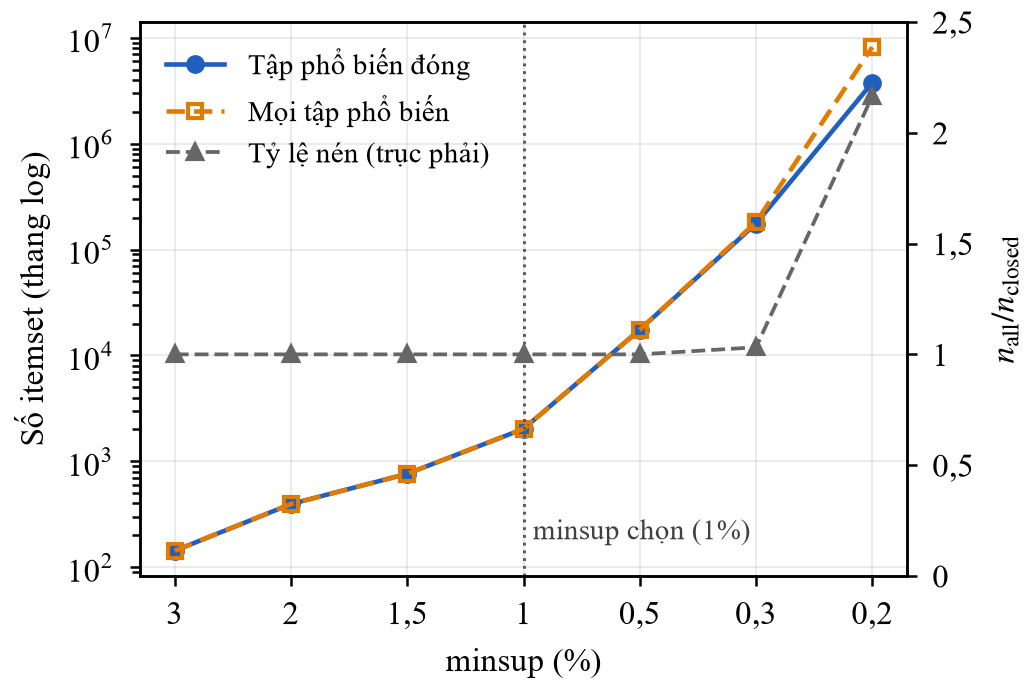
\includegraphics[width=\columnwidth]{figures/app1_minsup_survey.png}
\caption{Số tập phổ biến đóng, số mọi tập phổ biến (trục trái, thang log) và tỷ lệ nén
$n_{\mathrm{all}}/n_{\mathrm{closed}}$ (trục phải) theo minsup trên UCI Online Retail. Hai đường số tập trùng nhau từ
3\% đến 0,5\%; vạch chấm đánh dấu minsup được chọn.}
\label{fig:app1-minsup}
\end{figure}

Vì sản phẩm phổ biến nhất chỉ có support 11,5\%, minsup được khảo sát trong khoảng 3\% đến 0,2\%
(Hình~\ref{fig:app1-minsup}). Từ 3\% xuống 0,5\%, số tập đóng tăng từ 143 lên 17\,498 và luôn bằng số tập phổ biến:
trên dữ liệu thưa này, hầu như không có tập nào mà mọi hóa đơn chứa nó đều chứa thêm một sản phẩm chung khác. Tỷ lệ nén
chỉ vượt 1 ở 0,3\% (1,03) và đạt 2,16 ở 0,2\%. Từ 0,3\% xuống 0,2\%, số tập đóng tăng khoảng 21 lần, từ 176\,102 lên
3\,771\,107. Để kiểm tra ảnh hưởng của hóa đơn rất dài, nhóm chạy lại sau khi bỏ hóa đơn theo hai ngưỡng độ dài. Ngưỡng
500 sản phẩm chỉ bỏ 49 hóa đơn (0,25\% số giao dịch), nên dùng để hỏi liệu một nhóm rất nhỏ có đủ gây ra bước nhảy hay
không: số tập đóng ở 0,2\% giảm còn 424\,270, tức khoảng 88,7\%. Số tập đóng ở mức này vì vậy rất nhạy với nhóm hóa
đơn cực dài, dù kết quả không cho thấy mọi tập bị mất chỉ nằm trong các hóa đơn đó, vì việc bỏ hóa đơn cũng làm thay
đổi tập nào là tập đóng. Ngưỡng 200 sản phẩm bỏ 236 hóa đơn (1,2\%) và làm số tập đóng ở 1\% giảm từ 2\,026 xuống
1\,267, so với 1\,668 khi dùng ngưỡng 500; vì đây là phép thử chặt hơn trong hai ngưỡng, nó được dùng để kiểm tra độ ổn
định của luật trong phần kết quả luật bên dưới. Nhóm chọn minsup 1\%
để sinh luật, vì mỗi mẫu dựa trên ít nhất 198 hóa đơn và số tập phổ biến vừa phải (2\,026, trong đó 1\,197 tập có từ hai
sản phẩm); các mức dưới 1\% chỉ dùng để khảo sát. Ngưỡng confidence được đặt là $\mathit{minconf} = 0{,}6$.

Ở minsup 1\% (198 giao dịch), FPClose tìm được 2\,026 tập đóng, đúng bằng số tập phổ biến sau khôi phục, và bước sinh
luật cho 574 luật. Như vậy, ở cấu hình này biểu diễn tập đóng \emph{không đem lại lợi ích nén} (tỷ lệ nén 1,0); lợi ích
đó chỉ xuất hiện từ minsup 0,3\% trở xuống. Quy trình vẫn đáp ứng mục tiêu ứng dụng, vì luật được sinh từ mọi tập phổ
biến khôi phục đầy đủ từ tập đóng. Thời gian khai thác khoảng 0,4--0,5\,s, khoảng 3\,s nếu tính cả thời gian khởi động Julia. Để kiểm
tra độc lập với FPClose, support, confidence và lift của cả 574 luật được tính lại bằng phép đếm trực tiếp trên tập giao
dịch; 574/574 luật khớp, với sai số dưới $10^{-9}$. Phép kiểm này xác nhận các luật được sinh ra là đúng, nhưng không
chứng minh tập luật là đầy đủ; tính đầy đủ dựa trên việc tập phổ biến đã được đối chiếu với SPMF
(Mục~\ref{sec:correctness}) và bộ kiểm thử của bước sinh luật (Mục~\ref{sec:tests}).

\subsubsection{Kết quả luật}
Bảng~\ref{tab:app1-top10} trình bày mười luật có lift cao nhất. Cả mười luật đều thuộc bộ que cắm cây gia vị HERB MARKER,
với lift từ 76,8 đến 78,8 và confidence từ 0,83 đến 0,95: trong các hóa đơn chứa vế trái, tỷ lệ chứa vế phải cao gấp gần
80 lần tỷ lệ chung. Support chỉ từ 1,01\% đến 1,12\% (200--221 hóa đơn), sát ngưỡng minsup. Các luật đi theo cặp đối
xứng có cùng lift, vì $\mathrm{lift}(A \rightarrow B) = \mathrm{lift}(B \rightarrow A)$; tám luật đầu được tách từ hai
tập ba sản phẩm $\{$Thyme, Rosemary, Parsley$\}$ và $\{$Thyme, Rosemary, Basil$\}$. Khi bỏ 236 hóa đơn có từ 200 sản
phẩm trở lên (1,2\% số giao dịch), số luật ở minsup 1\% giảm từ 574 xuống 296, và 8/10 luật của
Bảng~\ref{tab:app1-top10} không còn đạt ngưỡng; chỉ cặp Thyme $\leftrightarrow$ Rosemary còn lại, với lift tăng từ 76,8
lên 85,0.

Vì top-10 theo lift bị một dòng sản phẩm chi phối, nhóm lập thêm Bảng~\ref{tab:app1-diverse} để bổ sung, không thay thế
Bảng~\ref{tab:app1-top10}. Các luật được duyệt theo đúng thứ tự xếp hạng của toàn bộ 574 luật, và một luật chỉ được nhận
khi không có sản phẩm nào của nó đã xuất hiện trong các luật đã nhận; cách lọc này chỉ chọn lại trong các luật FPClose đã
sinh ra. Mười luật trải trên nhiều dòng sản phẩm, với lift từ 38,4 đến 78,8 và confidence từ 0,65 đến 0,87. Vì phép lọc
chỉ bảo đảm không trùng mã sản phẩm, một số dòng xuất hiện ở hai luật (như HERB MARKER và Regency). Khi bỏ hóa đơn từ 200 sản
phẩm, sáu luật vẫn đạt ngưỡng và có lift tăng, còn bốn luật (hai luật HERB MARKER, đồ trang trí gỗ và hũ mứt) không còn
đạt. Ở minsup 2\%, chỉ còn 30 luật (30/30 khớp phép đếm trực tiếp), và không luật nào của Bảng~\ref{tab:app1-diverse} đạt
ngưỡng này, vì support của chúng chỉ từ 1,03\% đến 1,29\%. Luật đứng đầu ở 2\% thuộc bộ tách trà Regency, với support
2,74\% và lift 18,2: các luật ở ngưỡng cao hơn thuộc các bộ sưu tập bán chạy hơn và có lift thấp hơn, nhưng vẫn nối các
biến thể của cùng một bộ sưu tập.

\subsubsection{Ý nghĩa kinh doanh và giới hạn}
Các luật nổi bật chủ yếu nối các biến thể khác màu hoặc khác mẫu của cùng một bộ sưu tập: que cắm theo loại cây, đĩa trà
và bộ bát đường, bình sữa Regency theo màu, các phòng của bộ đồ chơi Poppy's Playhouse, cốc và bát chấm bi, dao nĩa trẻ
em theo mẫu. Từ đó nhóm nêu một số \emph{đề xuất chưa được kiểm chứng}. Thứ nhất, khi khách chọn một biến thể, hệ thống
có thể gợi ý các biến thể còn lại của bộ sưu tập; nên ưu tiên thử với sáu luật của Bảng~\ref{tab:app1-diverse} vẫn đạt
ngưỡng khi bỏ hóa đơn rất dài. Thứ hai, các mẫu chỉ đạt ngưỡng nhờ hóa đơn rất dài (trọn bộ HERB MARKER, đồ trang trí gỗ,
hũ mứt) phù hợp hơn với gói sản phẩm cho đơn hàng số lượng lớn. Thứ ba, luật có lift cao nhưng support khoảng 1\% hợp với
gợi ý nhắm đúng khách hàng, còn luật có support cao hơn như ở minsup 2\% hợp với khuyến mãi diện rộng. Hiệu quả của các
đề xuất này cần được đo bằng thử nghiệm A/B trước khi áp dụng.

Kết quả có các giới hạn sau. Luật chỉ phản ánh sự đồng xuất hiện trong cùng hóa đơn, không phải quan hệ nhân quả hay
thứ tự mua. Dữ liệu không ghi loại khách hàng, nên độ dài hóa đơn chỉ là dấu hiệu gián tiếp của đơn bán sỉ. Mỗi biến thể
là một StockCode riêng, nên luật chủ yếu nối các biến thể cùng dòng và ít cho thấy quan hệ giữa các dòng sản phẩm khác
nhau. Số lượng, đơn giá và thời gian mua chưa được dùng, nên luật chưa phản ánh doanh thu hay mùa vụ; dữ liệu cũng chỉ
thuộc một cửa hàng tại Vương quốc Anh trong giai đoạn 2010--2011.

\subsection{Ứng dụng 2: Khai thác mẫu trực quan trên ảnh}
\label{sec:app2}

\subsubsection{Bài toán và dữ liệu}
Ứng dụng tìm các tổ hợp từ thị giác (\textit{visual words}) phổ biến trong từng lớp ảnh, khảo sát chúng mô tả
vật thể hay vùng nền, và thử sử dụng chúng làm đặc trưng phân loại. Nhóm dùng Caltech-101~\cite{caltech101},
chọn năm lớp airplanes, Motorbikes, Faces\_easy, watch và Leopards. Mỗi lớp lấy 200 ảnh, chia phân tầng thành
140 ảnh train và 60 ảnh test, tổng cộng 700/300 ảnh; seed bằng 42. Các lớp có hình dạng và kết cấu khác nhau,
thuận tiện cho việc quan sát mẫu. Đây là nghiên cứu trường hợp trên năm lớp, không phải đánh giá toàn bộ
Caltech-101. Không dùng Faces để tránh trùng với Faces\_easy, hoặc lớp nền BACKGROUND\_Google.

\subsubsection{Biến đổi ảnh thành giao dịch}
Ảnh được chuyển sang mức xám, giữ tỉ lệ khi resize cạnh dài về 400 pixel. SIFT~\cite{lowe2004} được cấu hình
\texttt{nfeatures=500}; lưu descriptor cùng tọa độ keypoint để đối chiếu mẫu với ảnh. Bộ ảnh cho 449\,891 keypoint,
trong đó 315\,643 thuộc train. Nhóm lấy khoảng 150\,000 descriptor train, giới hạn tối đa 221 descriptor mỗi ảnh
để giảm sự áp đảo của ảnh nhiều keypoint, rồi học codebook bằng MiniBatchKMeans với $k\in\{100,300\}$,
\texttt{n\_init=3}, \texttt{batch\_size=4096}, seed 42. Mỗi descriptor được gán vào tâm gần nhất theo khoảng
cách Euclid. Codebook chỉ học trên train; test dùng lại các tâm đã học.
SIFT và k-means phụ thuộc nền tảng: cùng mã nguồn, seed và phiên bản thư viện, chạy trên Colab (Linux) cho cùng
vị trí keypoint với máy Windows dùng cho báo cáo nhưng descriptor khác (chỉ 28,8\% keypoint trùng descriptor); với
cùng đầu vào, codebook $k=100$ trùng từng byte còn $k=300$ khác (ARI 0,33, inertia lệch +0,07\%). Vì vậy notebook dùng lại đặc trưng SIFT, codebook
và phép gán từ đã lưu của lần chạy chính (kiểm tra SHA-256) để tái lập đúng số liệu; SIFT và k-means vẫn được tính
lại trên máy đang chạy trong các ô kiểm chứng để so với bản đã lưu.

Gọi $n_i(w)$ là số keypoint của ảnh $i$ được gán vào từ $w\in\{0,\ldots,k-1\}$. Giao dịch của ảnh là
\begin{equation}
T_i=\{w+1\mid n_i(w)\geq\tau,\ w\notin S\},\qquad \tau=3,
\label{eq:app2-transaction}
\end{equation}
trong đó $S$ gồm các từ có mặt, sau ngưỡng $\tau$, trong hơn 80\% ảnh train. Item được cộng 1 để có mã dương,
sắp tăng và không lặp khi xuất định dạng SPMF. Mỗi giao dịch ghi nhận sự đồng xuất hiện trên toàn ảnh,
không khẳng định các từ kề nhau hay tạo thành một bộ phận vật thể.

Ngưỡng $\tau$ được chọn theo quy tắc định trước: với stop word 80\%, lấy $\tau$ lớn nhất trong $\{1,2,3\}$
có accuracy CV 5-fold trên train không thấp hơn mức tốt nhất quá 0,01. Mô hình dùng để chọn là Logistic
Regression trên vector hiện diện từng item, không phải vector mẫu khai thác. Cả hai codebook chọn $\tau=3$.
Đây là chỉ báo nội bộ: codebook và stop word được học trên toàn bộ train trước khi chia fold, nên chưa phải
CV của toàn pipeline. Tập test cuối không tham gia lựa chọn này.

Không có giao dịch rỗng ở cấu hình đã chọn. Độ dài trung bình trên train là 57,0 item với $k=100$ và 58,1
với $k=300$; riêng airplanes chỉ đạt 37,7 và 31,5. Stop word loại tương ứng một và không từ, do đó tác động
lọc trong cấu hình này rất nhỏ. Các bước trên được cài trong notebook và các script phụ trợ; OpenCV và
scikit-learn phục vụ trích đặc trưng, gom cụm và đánh giá, còn khai thác tập phổ biến dùng cài đặt của nhóm.

\begin{figure*}[!t]
\centering
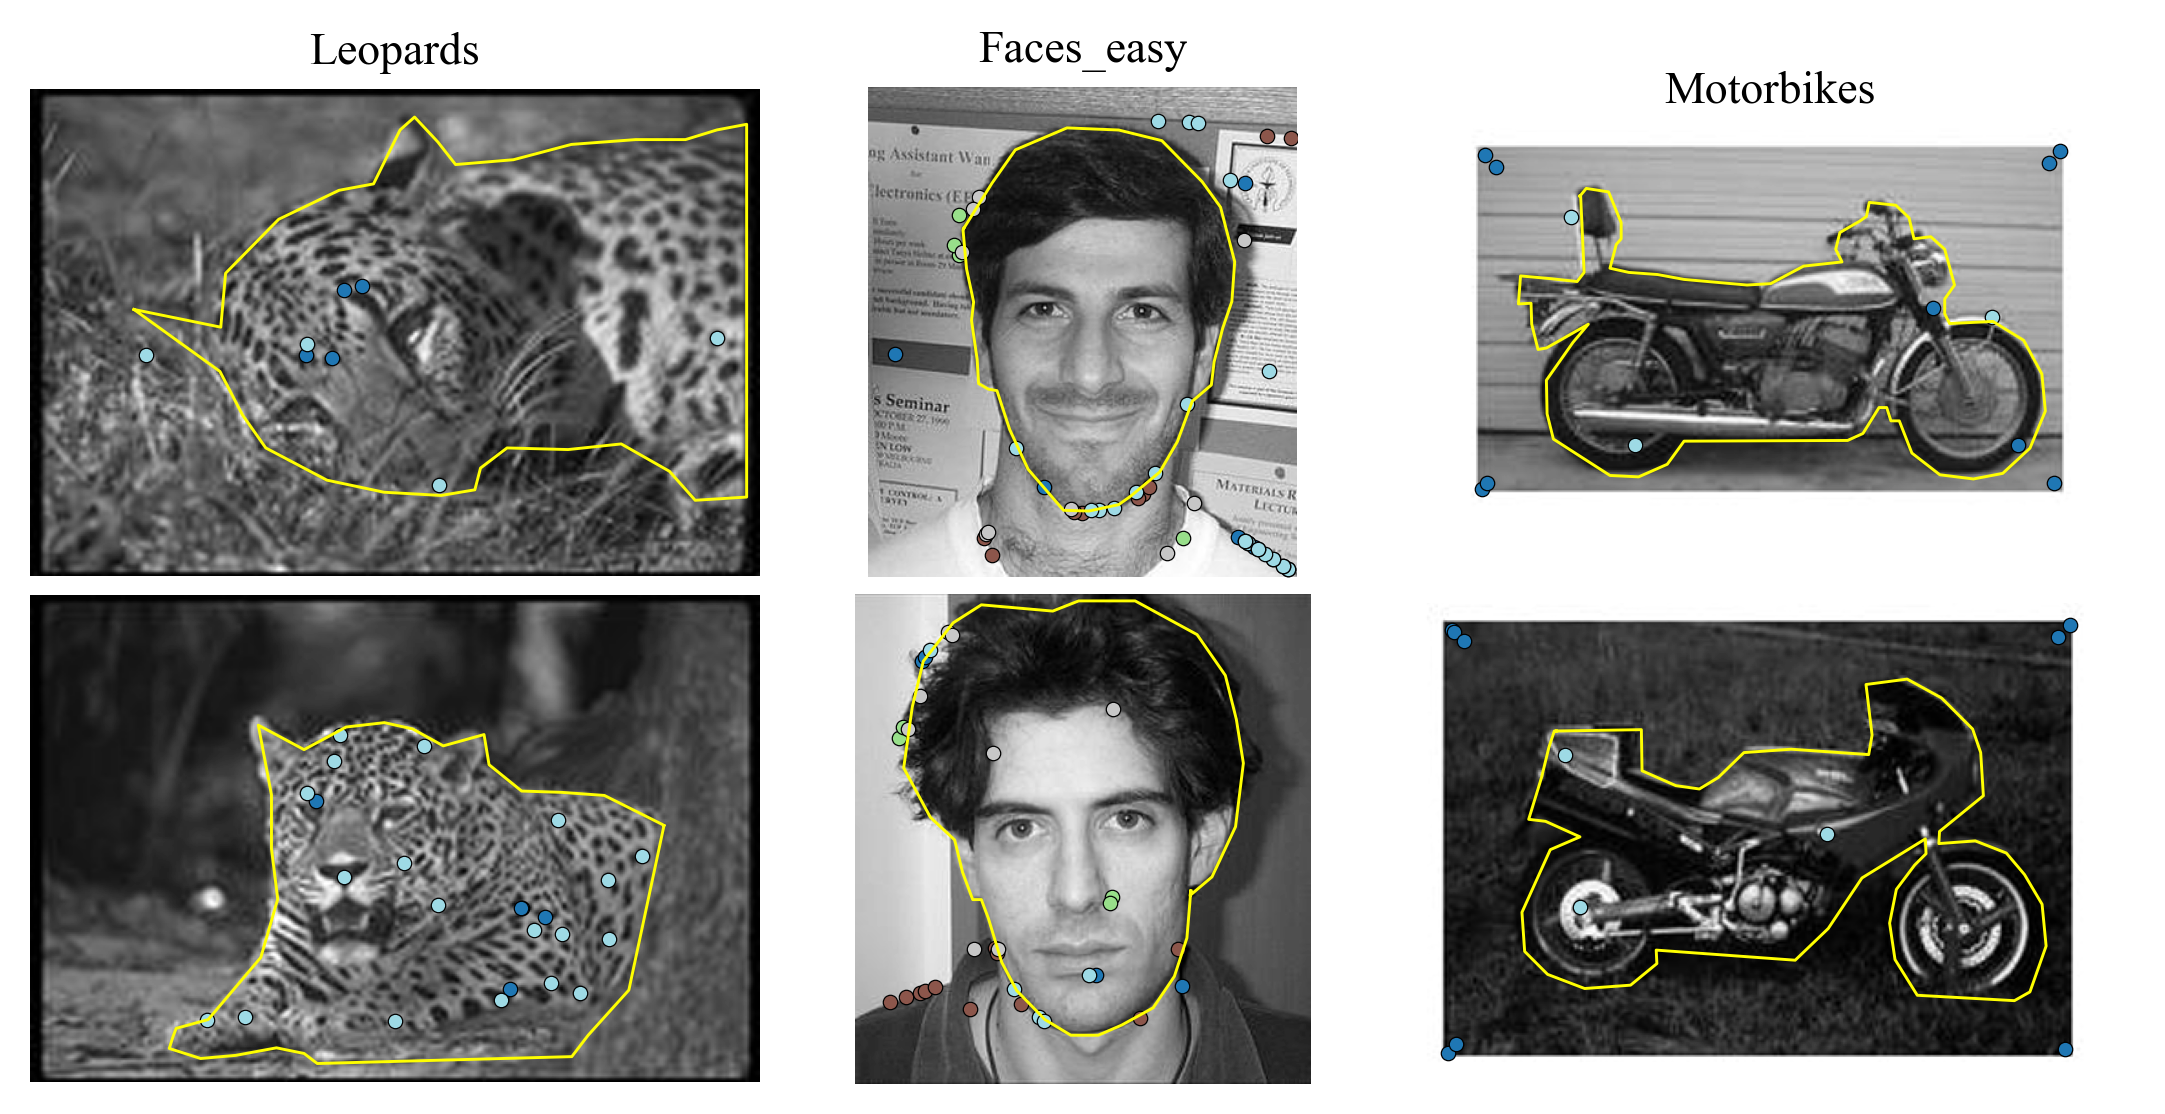
\includegraphics[width=0.92\textwidth]{figures/app2_patterns.png}
\caption{Mẫu top-1 tại $k=300$ của ba lớp Leopards, Faces\_easy và Motorbikes, mỗi lớp hai ảnh train
lấy từ bộ ảnh minh họa chọn bằng seed 42.
Chấm màu là tâm keypoint mang từ thuộc mẫu; cùng màu biểu diễn cùng từ trong mỗi lớp; đường vàng là contour
vật thể. Các ảnh chỉ minh họa, còn tỷ lệ ở Bảng~\ref{tab:app2-top} dùng mọi ảnh train chứa mẫu.}
\label{fig:app2-patterns}
\end{figure*}

\subsubsection{Khai thác và lựa chọn mẫu}
Nhóm gọi FPClose Julia qua \texttt{demo.jl} riêng cho từng lớp, chỉ với giao dịch train. Kết quả là các tập
phổ biến đóng: không có tập cha thực sự nào cùng support. Biểu diễn này bảo toàn thông tin support của
các tập phổ biến trong cùng CSDL và ngưỡng; một tập phổ biến có support bằng support lớn nhất trong các
tập đóng chứa nó. Không dùng kết quả từ thư viện FIM có sẵn cho ứng dụng.

Với mỗi $k$, nhóm quét minsup giảm dần theo bước 5 điểm phần trăm và chọn mức cao nhất mà cả năm lớp đều
có ít nhất 50 tập đóng dài từ hai item. Ngưỡng chung cho phép đối chiếu các lớp dưới cùng yêu cầu support,
đồng thời cung cấp ứng viên cho top-10 phân tích và top-20 phân loại. Trước khi chốt quy tắc, nhóm đã chạy
thử mức 60\% trên ba file để xác định lưới quét. Kết quả chọn 55\% ($77/140$ ảnh) cho $k=100$ và 25\%
($35/140$ ảnh) cho $k=300$. Airplanes quyết định cả hai ngưỡng, với 63 và 102 tập dài từ hai item.

\begin{table}[!t]
\centering
\caption{Số tập phổ biến đóng theo lớp, gồm mọi độ dài.}
\label{tab:app2-counts}
\footnotesize
\begin{tabular}{lrr}\hline
Lớp & $k=100$, minsup 55\% & $k=300$, minsup 25\%\\\hline
airplanes & 77 & 132\\
Motorbikes & 86\,852 & 650\\
Faces\_easy & 124\,779 & 5\,963\\
watch & 2\,477 & 1\,145\\
Leopards & 381\,587 & 2\,604\,564\\\hline
\end{tabular}
\end{table}

Bảng~\ref{tab:app2-counts} cho thấy số mẫu chênh lệch rất lớn dù các lớp có cùng số giao dịch. Ngưỡng chung
bị lớp ít mẫu chi phối, khiến Leopards sinh hơn 2,6 triệu tập ở $k=300$. Số mẫu lớn không đồng nghĩa với
nhiều thông tin phân biệt độc lập. Nhóm đếm lại support của mọi tập đầu ra bằng bitset Python; tất cả
khớp. Tính đóng đúng trên các tập được kiểm tra, tối đa 5\,000 tập mỗi lớp; phép kiểm này không xác nhận
tính đầy đủ của đầu ra. Kiểm thử đối chiếu thuật toán với SPMF được trình bày ở các chương trước.

Để đo mức đặc trưng theo lớp, nhóm dùng growth rate (GR), theo ý tưởng emerging patterns~\cite{dong1999}:
\begin{equation}
\mathrm{GR}(X,c)=\frac{s_c(X)/140}{s_{\neg c}(X)/560},
\label{eq:app2-gr}
\end{equation}
với $s_c(X)$ và $s_{\neg c}(X)$ lần lượt là số ảnh train chứa trọn mẫu $X$ trong và ngoài lớp $c$.
Nếu $s_{\neg c}(X)=0$, đặt GR bằng $\infty$. Chỉ xét mẫu dài từ hai item, xếp theo GR giảm dần, rồi support
trong lớp giảm dần, độ dài giảm dần và chuỗi item để cố định thứ tự. GR vô cực chỉ cho biết mẫu chưa xuất
hiện trong 560 ảnh train ngoài lớp, không chứng minh lớp tách biệt hoàn toàn trên dữ liệu mới.

\subsubsection{Phân tích ý nghĩa các mẫu}
Với mỗi mẫu top-10, trên mọi ảnh train của lớp chứa mẫu, nhóm đếm tỷ lệ tâm keypoint mang từ thuộc mẫu
nằm trong contour vật thể (\textit{on\_object}). Baseline là tỷ lệ của mọi keypoint trong cùng các ảnh đó.
Hai tỷ lệ được tính bằng tổng số keypoint, không phải trung bình đều theo ảnh. Bảng~\ref{tab:app2-top}
trình bày mẫu đứng đầu mỗi lớp ở $k=300$; Hình~\ref{fig:app2-patterns} minh họa ba lớp tiêu biểu.

\begin{table}[!t]
\centering
\caption{Mẫu top-1 ở $k=300$. $s_c/s_{\neg c}$ là số ảnh chứa mẫu (mẫu số tương ứng 140/560);
$p/b$ là tỷ lệ on\_object/baseline. Các số trong $X$ là mã item SPMF.}
\label{tab:app2-top}
\scriptsize\setlength{\tabcolsep}{2.5pt}
\begin{tabular}{llrrr}\hline
Lớp & $X$ & $s_c/s_{\neg c}$ & GR & $p/b$\\\hline
airplanes & 17,62,254 & 37/44 & 3,36 & 0,185/0,297\\
Motorbikes & 123,127 & 42/3 & 56 & 0,439/0,779\\
Faces\_easy & 45,69,113,159,183 & 35/2 & 70 & 0,256/0,394\\
watch & 45,186,205,230 & 35/5 & 28 & 0,938/0,943\\
Leopards & 156,263 & 100/0 & $\infty$ & 0,940/0,749\\\hline
\end{tabular}
\end{table}



\textbf{Leopards.} Trung bình on\_object của top-10 là 0,949 so với baseline 0,761. Hình cho thấy các
keypoint tập trung trên lông báo, phù hợp với giả thuyết mẫu mô tả kết cấu đốm. Ở $k=300$, 2\,582\,554
trong 2\,604\,468 mẫu dài từ hai item có GR vô cực (99,16\%), nên GR không phân biệt được chúng và support
trở thành tiêu chí xếp hạng tiếp theo. Mẫu top-1 phủ 100/140 ảnh Leopards, không phải toàn bộ lớp.
Quan sát vị trí của các mẫu top chưa đủ để xác định nguyên nhân bùng nổ tổng số tập đóng.

\textbf{Faces\_easy và Motorbikes.} Top-10 Faces\_easy có on\_object trung bình 0,267, thấp hơn baseline
0,422; nhiều điểm nằm ở nền và sát đường viền tóc, cằm. Với Motorbikes, mẫu top-1 có GR 56 nhưng tỷ lệ
trên vật thể chỉ 0,439 so với baseline 0,779; các điểm xuất hiện ở góc ảnh lẫn trên xe. Vì vậy, mẫu có GR
cao không nhất thiết mô tả bộ phận vật thể: thông tin nền hoặc biên ảnh cũng có thể gắn với lớp.
Đây là bằng chứng về vị trí mẫu, chưa phải kiểm chứng nhân quả rằng bộ phân loại dựa vào nền.

\textbf{Airplanes và watch.} Top-10 airplanes có GR khoảng 2,37--3,36 tại $k=300$, cho thấy khả năng
phân biệt hạn chế trong các mẫu được xét; hình minh họa đầy đủ trong notebook cho thấy nhiều điểm ở mép
ảnh và đường băng. Với watch, on\_object của top-1 gần baseline (0,938 so với 0,943): vật thể chiếm phần
lớn ảnh, nên tỷ lệ nằm trong contour cao tự nó chưa chứng minh mẫu tập trung vào vùng đặc biệt.

\subsubsection{Đánh giá phân loại và giới hạn}
Nhóm so sánh ba biểu diễn với cùng StandardScaler học trên train và Logistic Regression
(\texttt{max\_iter=5000}, seed 42): A là histogram BoVW chia cho tổng keypoint của ảnh; B là 100 đặc trưng
nhị phân từ top-20 mẫu mỗi lớp, bằng 1 khi ảnh chứa trọn mẫu; C nối A và B. Test chỉ được gán từ và kiểm tra
chứa mẫu, không tham gia khai thác hoặc xếp hạng mẫu. Bảng~\ref{tab:app2-classify} báo cáo kết quả trên cùng
300 ảnh test; confusion matrix và recall từng lớp có trong notebook.

\begin{table}[!t]
\centering
\caption{Phân loại trên 300 ảnh test. A: BoVW; B: mẫu; C: A+B.}
\label{tab:app2-classify}
\footnotesize
\begin{tabular}{crrrr}\hline
$k$ & Biểu diễn & Số chiều & Accuracy (\%) & Macro-F1\\\hline
100 & A & 100 & 82,33 & 0,8228\\
100 & B & 100 & 67,00 & 0,6635\\
100 & C & 200 & 82,33 & 0,8236\\\hline
300 & A & 300 & 87,00 & 0,8712\\
300 & B & 100 & 60,33 & 0,6064\\
300 & C & 400 & 87,67 & 0,8773\\\hline
\end{tabular}
\end{table}

B thấp hơn A khoảng 15--27 điểm phần trăm. Điều kiện chứa trọn mẫu làm mất độ phủ: 15/300 ảnh test ở
$k=100$ và 49/300 ở $k=300$ có vector B toàn 0, nên không thể phân biệt các ảnh này bằng B. A vẫn sử dụng
phân bố của mọi từ, còn B bỏ tần suất và các từ ngoài bộ mẫu. Một số nhóm mẫu cũng chia sẻ nhiều item;
tuy nhiên, chưa có thí nghiệm tách riêng ảnh hưởng của độ dư thừa, độ phủ và thông tin nền. C bằng A về
accuracy ở $k=100$ và hơn hai dự đoán đúng ở $k=300$. Chưa có bằng chứng rõ về lợi ích phân loại của
cách chọn và biểu diễn mẫu này; kết luận không áp dụng cho mọi cách sử dụng tập phổ biến.

Kết quả chỉ dựa trên một lần chia train/test. Khoảng tin cậy accuracy trong notebook không đo biến thiên
do đổi tập huấn luyện và không thay thế phép so sánh ghép cặp giữa các mô hình. Phép đo vị trí chỉ xét
tâm keypoint, trong khi vùng descriptor có thể cắt qua contour. Ngoài ra, resize chủ yếu phóng to ảnh,
đặc biệt Leopards khoảng 2,1 lần; khác biệt độ phân giải theo lớp có thể ảnh hưởng visual words.
Tính lại SIFT và học lại k-means trên Colab cho số liệu khác: minsup chọn cho $k=300$ là 20\% thay vì 25\%; ở $k=100$ quy tắc chọn
minsup không đạt (airplanes chỉ có 42 tập ở 55\%, còn ở 50\% Leopards vượt giới hạn 300 giây); số tập đóng chênh
đáng kể và accuracy lệch 0,3--3 điểm phần trăm. Các kết luận định tính (vị trí mẫu theo lớp, B thấp hơn A, C xấp xỉ
A) không đổi; các con số cụ thể gắn với codebook đã chọn.
Trong phạm vi khảo sát, đóng góp rõ nhất của mẫu là hỗ trợ phân tích các tổ hợp đặc trưng và chỉ ra
sự hiện diện của thông tin nền/biên ảnh mà một con số accuracy không thể diễn tả.
